\documentclass[convert]{standalone}

\usepackage{tikz}
\pagestyle{empty}

% INT_AY22_L03_Fig02_Moving_ball_w_displ.png

\begin{document}
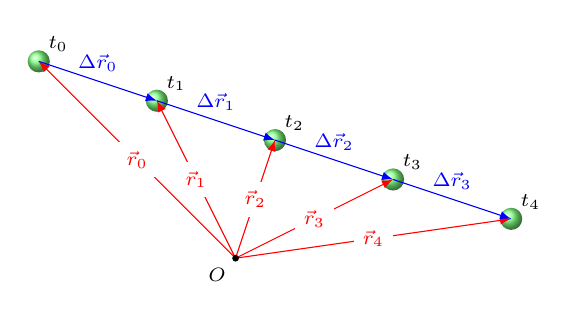
\begin{tikzpicture}[> = latex, font = \scriptsize]

	% Definitions
	
	\def\xi{-2.5}		% Initial x, y coordinates
	\def\yi{2.5}
	
	\def\vx{1.5}		% Velocity components
	\def\vy{-0.5}
	
	% Draw ball
	
	\foreach \n in {0, 1, ..., 4}
	{
		\draw [ball color = green!50, draw = none] ({\xi + \n * \vx}, {\yi + \n * \vy}) circle (4 pt) node [above right] {$t_\n$};
		\draw [->, red] (0, 0) -- node [midway, fill = white] {${\vec r}_\n$} ({\xi + \n * \vx}, {\yi + \n * \vy});
	}
	
	\foreach \n in {0, 1, ..., 3}
		\draw [->, blue] ({\xi + \n * \vx}, {\yi + \n * \vy}) -- node [above] {$\Delta {\vec r}_\n$} ({\xi + (\n + 1) * \vx}, {\yi + (\n + 1) * \vy});
	
	% Draw origin
	
	\filldraw (0, 0) circle (1 pt) node [below left] {$O$};
	
\end{tikzpicture}
\end{document}